\section{シナリオモジュール}
\label{sec:scenario}
シナリオモジュールについて述べる.
シナリオモジュールはトポロジカルマップから作成されたシナリ
オから「突き当りまで」という「条件」や「左折」なとの「行動」を解釈し,
単語で構成された経路を分岐路での目標方向へ変換して出力する.

\figref{fig:topo2sce}にトポロジカルマップとそれをもとに作成されるシナリオを示す.
図の例では出発地点をエッジ2,目的地をノード2として,その間のエッジとノードを移動する.
エッジ2からノード1は「三叉路まで」という条件と「直進」という行動,
ノード1からエッジ1は「右折」という行動,
エッジ1からノード2は「突き当り(三叉路)まで」という条件と「直進」の行動で表現される.
これらを統合すると,
最終的に「三叉路まで直進.右折.突き当たりまで直進.停止.」
のシナリオが作成される.

次に作成したシナリオを目標方向に変換する処理を述べる.
はじめにシナリオを句点ごとに分解し,部分シナリオというものを作成する.
この部分シナリオには,次の部分シナリオに遷移するための「条件」とロボットが行う必要がある「行動」
が含まれている.
この部分シナリオを形態素分析(MeCab\cite{2004ConditionalRF})を用いて単語へ分割する.
分割した単語は,「条件」と「行動」を示す以下の項目に分けて登録される.
\begin{enumerate}
    \item [1)] 通路の特徴 例えば,「三叉路」「角」など
    \item [2)] 順番 例えば,「3 つ目の」「2 番目の」など 
    \item [3)] 方向 例えば,「左手に」「右手に」など
    \item [4)] 行動 例えば,「右折」「停止」など
\end{enumerate}
先に示した例は句点ごとに,
三叉路まで直進/ 
右折/   
突き当たりまで直進/  
停止/ 
と分解される.

1つ目の条件と行動は 
1)通路の特徴 三叉路,4)行動 直進,

2つ目の行動は 4)行動 右折となる.

3つ目の条件と行動は
1)通路の特徴 突き当たり 4)行動 直進

4つ目の行動は
4)停止となる.

この4)行動を\tabref{tab:target}で示したデータ形式で表現し,分岐路での目標方向として,経路追従モジュールへ与える.
ここで,「三叉路まで」といった条件を達成したかの判定は,
\secref{sec:intersection}の通路分類モジュールの分類結果を用いて行う.
\vspace{3zh}
\begin{figure}[htbp]
    \centering
     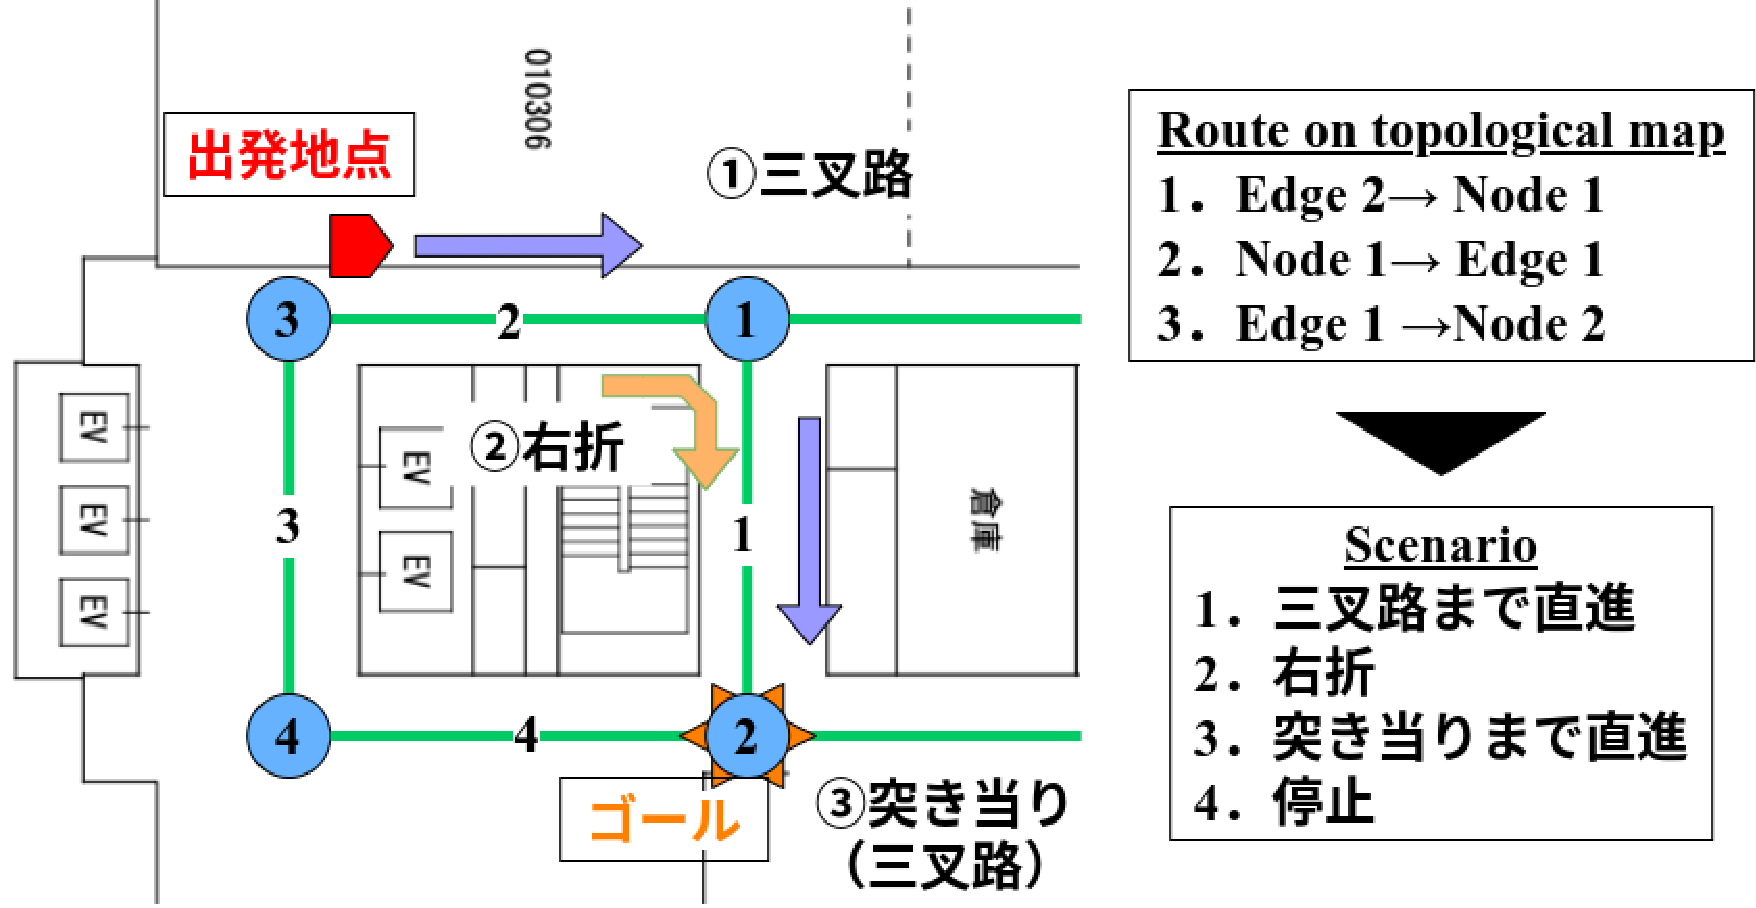
\includegraphics[width=90mm]{images/pdf/topo2sce.pdf}
     \caption[Example of topological map and created scenario]{Example of topological map and created scenario(Quoted from \cite{haruyama2023})}
     \label{fig:topo2sce}
\end{figure}